\section{Symmetry Breaking In 4-Connected Grid Maps}
\label{cha::rsr::symm4c}

As a first step, we will describe a simple technique for breaking path symmetries 
in the context of 4-connected grid maps.
This is a domain which appears regularly in the academic literature
\citep{yap02,wang08,pochter10} and is often found in the pathfinding systems of
modern computer games.  Some examples include Square Enix's \emph{Heroes of
Mana} (released in 2007 for the Nintendo DS), Astraware's \emph{My Little Tank}
(2008, iPhone) and Atari's \emph{Dragon Ball Z: Legacy of Goku} (2002, Gameboy
Advance). We propose the following strategy:

\begin{enumerate}
\item{Decompose the grid map into a set of empty rectangles, each of which contains no obstacles.}
\item{Prune all nodes from the interior but not the perimeter of each rectangle.}
\item{Add a series of \emph{macro edges} that connect each node on the perimeter of a rectangle
with a node from the directly opposite side\footnote{We can avoid storing
macro edges by generating them on-the-fly during search.}.  The cost of each
edge is equal to the Manhattan distance\footnote{Defined in
Chapter~\ref{cha::lit::heuristics}} between its two endpoints.
}
%\item{During search, temporarily re-insert tiles back into the map to handle cases where the
%start or goal is a location which has been previously pruned.}
\end{enumerate}

\begin{figure}[t]
\begin{center}
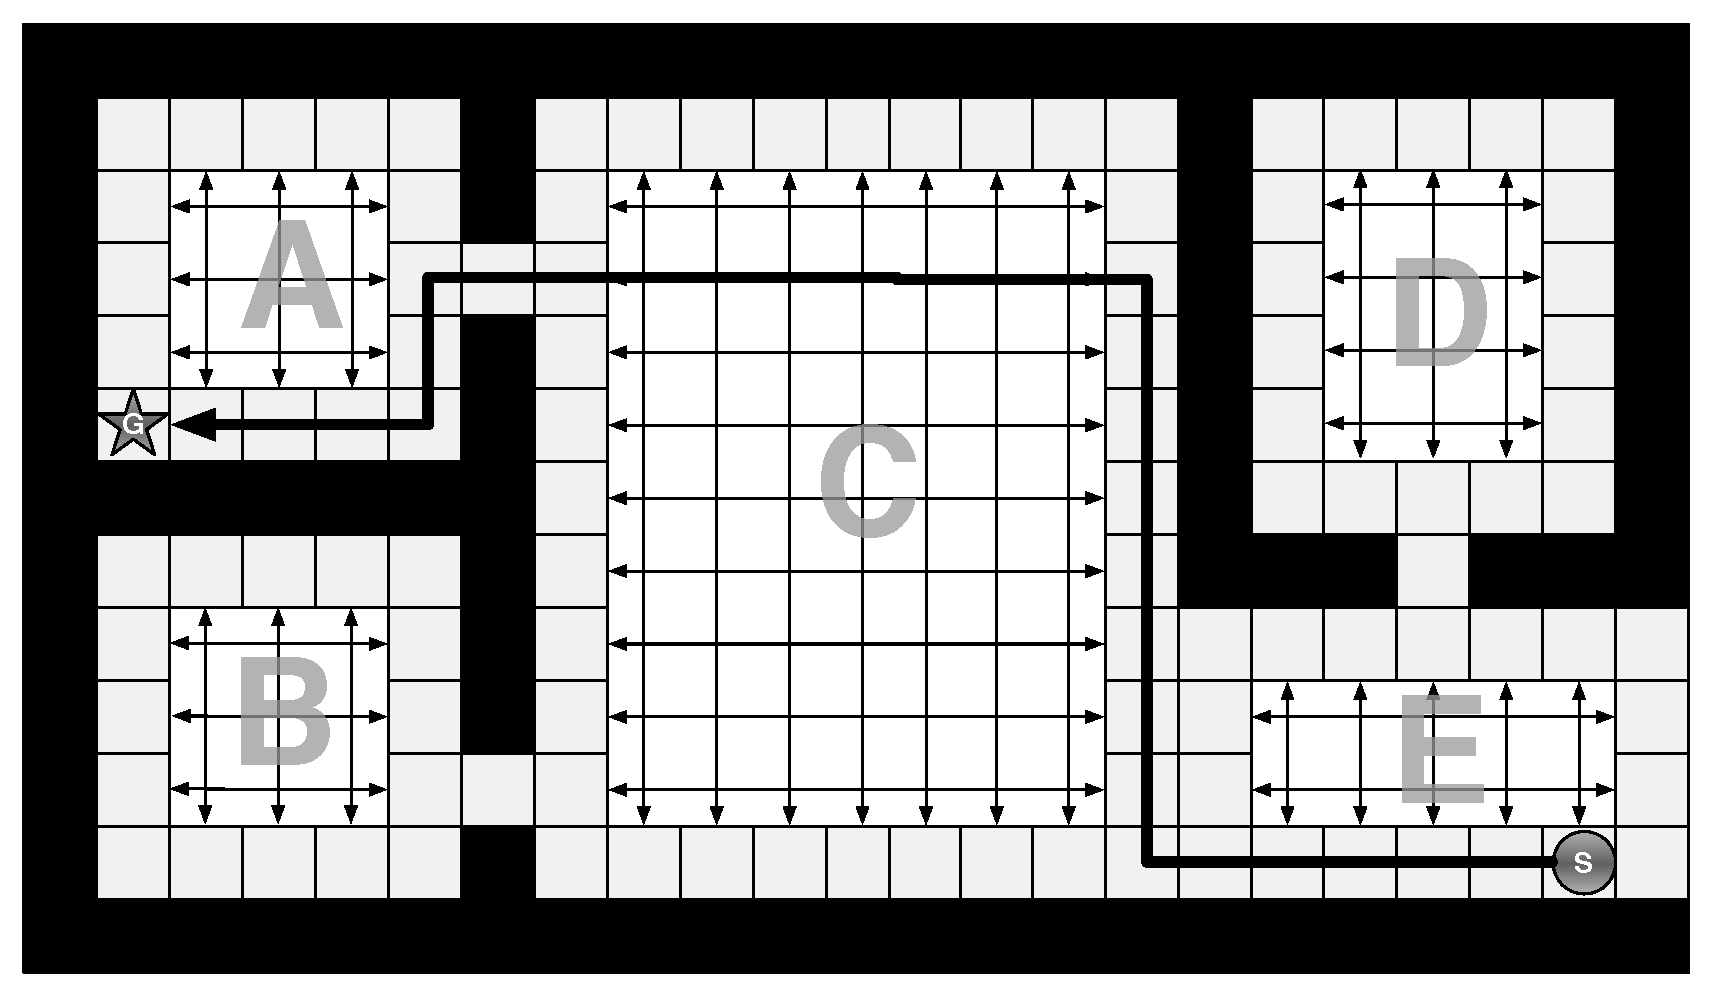
\includegraphics[scale=0.30, trim = 10mm 10mm 10mm 0mm]{chapter_rsr/diagrams/4c_example.pdf}
\end{center}
\vspace{-3pt}
\caption[Rectangular Symmetry Reduction on 4-connected maps]{
\small
RSR decomposes a grid map into a set of empty rectangles. 
Nodes interior to each rectangle are pruned leaving a set of perimeter nodes.
Macro edges are then added to facilitate optimal travel from one side of the perimeter to the other.}
\label{fig::rsr::overview}
\end{figure}

The decomposition of maps into empty rectangles involves a greedy flood-filling
strategy which we discuss in Section~\ref{cha::rsr::rectangles}. Note however
that rectangle sizes are not fixed and can vary across a map depending on the
placement of obstacles.  Trivial rectangles which contain no interior nodes (for
example those with a width $w$ or height $h$ $\leq 2$) are left unmodified by
steps 2 and 3.  Figure \ref{fig::rsr::overview} shows an example of this process.  For
each non-trivial rectangle we prune $(w-2)\times(h-2)$ interior nodes and, in
the process, eliminate a large number of symmetric paths between nodes on the
perimeter.  We claim that this approach preserves optimality when traversing
across any arbitrary rectangle.

\begin{lemma}
\label{thm::rsr::rectangletraversal}
Let $R$ be an arbitrary rectangle that is free of obstacles
and $m, n$ be two locations on its perimeter.
Then $m$ and $n$ can be connected optimally through a path that
mentions only nodes on the perimeter of $R$ and possibly involves
a macro edge.
\end{lemma}
\begin{proof}
\par
There are two distinct cases to consider.
Case 1 is when $m$ and $n$ are placed on the same side of the perimeter, or
on two orthogonal sides. 
To obtain an optimal path we can simply travel along the perimeter from $m$ to $n$.
Case 2 is when $m$ and $n$ are placed on opposite sides of the perimeter.
To obtain an optimal path we can simply follow the macro edge at $m$ 
and navigate directly to a node $m'$ located on
the same side of the perimeter as $n$. Then, go from $m'$ to $n$ along the perimeter.
The resultant path is optimal as its length is equal to the Manhattan distance between $m$ and $n$.
\end{proof}

A direct corollary to Lemma \ref{thm::rsr::rectangletraversal} is that we can prune from consideration
all nodes from the interior of $R$ and limit ourselves to only searching nodes appearing along its perimeter. 
The only remaining consideration is how to deal with interior nodes that happen
to be the start or goal location for the search at hand.
We address this case in the following section.

\subsection{Online Insertion}
\label{cha::rsr::insertion}
Often an interior node pruned as a result of offline symmetry elimination
is required as a start or goal location for an agent.
We handle such cases by inserting back into the graph interior start and goal nodes  
for the duration of the search.
We use the following procedure (highlighted in Figure \ref{fig::rsr::insertion}):
\begin{enumerate}
\item{If the start and goal are in the same rectangle no insertion is required.
 Since it is guaranteed that there are no obstacles between the two locations, an optimal 
 path is trivially available. This case will be ignored in the rest of our discussion.}
% take the Manhattan distance between them as the length of the optimal path. }
\item{If the start and goal are not in the same rectangle, connect each of them
to the closest neighbours on each side of the perimeter of the empty rectangle.}
\end{enumerate}
We claim that this procedure retains optimality when searching from the start (or goal) location
to all nodes on the perimeter of its rectangle.

\begin{figure}[t]
	\vspace{-4pt}
       \begin{center}
           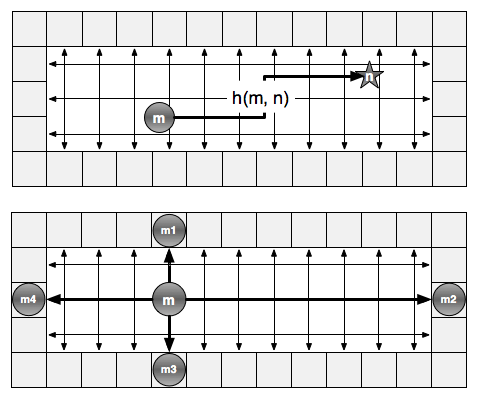
\includegraphics[scale=0.50, trim = 10mm 10mm 10mm 0mm]{chapter_rsr/diagrams/roomtraversal.png}
       \end{center}
	\vspace{-3pt}
\caption[Examples of online insertion]
{\small
(Top) When $m$ and $n$ are in the empty rectangle no insertion (or search) is necessary.
(Bottom) $m$ is a previously pruned interior node.
We insert $m$ into the graph and connect it to neighbours on each side of the empty rectangle.}
%\vspace{-15pt}
	\label{fig::rsr::insertion}
\end{figure}

\begin{lemma}
\label{thm::rsr::insertion}
Let $R$ be an empty rectangular rectangle.
For any nodes $m, n$, with $m$ a re-inserted interior node and $n$ a node on the perimeter,
it is always possible to find an optimal length path which mentions no interior nodes except for $m$.
\end{lemma}
\begin{proof}
We insert $m$ into the graph and connect it to $m'_{1}, m'_{2}, m'_{3},
m'_{4}$, the closest neighbours on each side of the perimeter.  The weight of
each edge incident with $m$ is equal to the straight-line distance between $m$
and each $m'_{i}$.  To find an optimal path to $n$ we travel from $m$ to the
node $m'_{i}$ which is on the same side as $n$ on the perimeter.  From there
we travel along the perimeter of $R$ until we reach $n$.
%\par
%Next, suppose $s, g \in N$. 
%In this case we do not insert anything; the length of the optimal path is equal
%to the Manhattan distance between $s$ and $g$.
\end{proof}

Once the search has finished we remove the start and goal from the graph.
The time required in each case (insertion and deletion) is constant.

\subsection{Optimality}
\label{char::rsr::optimal4c}
We claim that A*, when applied to a 4-connected grid map pruned by RSR, 
will always return an optimal solution if one exists.

\begin{theorem}
\label{thm::rsr::optimality}
For every optimal length path $\pi^*(s, g)$ in a 4-connected grid map there exists
an equivalent length path in the pruned version of the grid map.
\end{theorem}
\begin{proof}
Follows from Lemma \ref{thm::rsr::rectangletraversal} and Lemma \ref{thm::rsr::insertion}.
For every optimal length segment of $\pi^{*}(s, g)$ which traverses
through an empty rectangle, from a perimeter node $m$ to a perimeter node $n$, 
there is an equivalent segment which mentions only nodes
on the perimeter of that rectangle (and possibly one macro-step).
\end{proof}

A direct corollary of Theorem \ref{thm::rsr::optimality} is that optimal
solutions pruned by our symmetry reduction can be easily reconstructed; for
example to avoid unnatural looking paths where agents seem to hug walls.
Consider a path fragment between $m$ and $n$, two nodes on the perimeter of an
empty rectangle.  Assume, without any generality loss, that the path fragment
contains $r$ moves to the right and $u$ moves upwards.  All optimal path
fragments between $m$ and $n$ can be obtained by interleaving $r$ moves to the
right and $u$ moves upwards in any order (e.g right-right-up, right-up-right,
up-right-right).


\begin{figure}[t]
%	\vspace{-4pt}
\centering
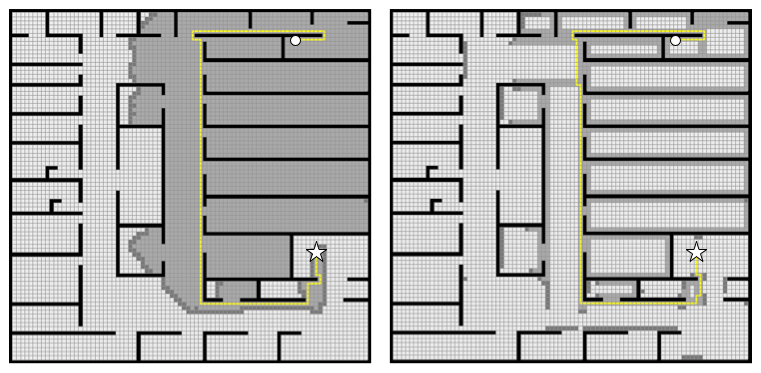
\includegraphics[width=0.95\columnwidth, trim = 10mm 10mm 10mm 0mm]{chapter_rsr/diagrams/rsr_example.png}
\caption[Searching with A{*} vs. A{*} + RSR] 
{\small
(Left) A* solving a problem on an unmodified ($86\times88$) grid map. 
Expanded nodes are marked dark grey.
(Right) A* solving the same problem using our modified grid map. 
The algorithm only considers nodes along the perimeter of the identified rectangles.}
\label{fig::rsr::contrast}
\end{figure}

In Figure \ref{fig::rsr::contrast} we highlight the effectiveness of our
symmetry breaking technique using a map that has characteristics similar to
what one might expect in a modern role-playing game\footnote{In fact, many
computer game maps tend to be somewhat bigger than our example but for
demonstration purposes it is sufficient.}; i.e. there are many rooms with
entrances and corridors connecting them.  A* running on the original grid map
expands almost half the nodes in the state space of the shown example.  We
then apply our technique to eliminate symmetries and re-run A*.  This time A*
expands less than 15\% of all nodes (more than a three-fold improvement) and
returns an optimal solution 3 times faster.

\subsection{Identifying Empty Rooms}
\label{cha::rsr::rectangles}
In this section we give a simple but effective flood-fill-based algorithm for decomposing a 
grid map into empty rectangles.
We will try to build large rectangles before small ones and prefer rectangles which
contain as many interior nodes as possible:

\begin{enumerate}

\item{\label{rectanglesalg:step1} For each traversable tile $t$, build a maximal size empty
rectangle which has $t$ as its upper left corner. Each such rectangle should contain only
traversable tiles which have not already been assigned to a rectangle.}

\item{\label{rectanglesalg:step2} Using a Max-Heap, sort the list of traversable tiles using the number of
interior nodes in the rectangle of each $t$ as its priority.}

\item{\label{rectanglesalg:step3} Take from the heap the tile $t$ with highest priority
which has not already been assigned to a rectangle. }

\item{\label{rommsalg:step4} Verify the priority of $t$\footnote{Some of the tiles in the associated rectangle
may have been assigned to another rectangle since we added $t$ to the heap.} by building another maximal size
empty rectangle (as per Step \ref{rectanglesalg:step1}) which has $t$ as its upper
left corner and contains no obstacles or tiles already assigned to another rectangle.}

\item{\label{rectanglesalg:step5} If the number of interior nodes in the new rectangle is equal to the 
priority of $t$ we say that the rectangle forms a rectangle and add it to our decomposition. 
Otherwise, we update the priority of $t$ with the number of interior 
nodes contained in the new rectangle. }

\item{\label{rectanglesalg:step6} Repeat Steps \ref{rectanglesalg:step3} to \ref{rectanglesalg:step5} until the heap is
empty and all nodes have been assigned to a rectangle in the decomposition.}

\end{enumerate}

The construction of empty rectangles is similar to the computation of \emph{clearance
values} in \citep{harabor08}.  In that work the objective is to calculate the
amount of traversable space at any given location on the map.  This is achieved
by constructing maximum sized squares that originate at each traversable tile on
the map.  Our rectangle identification procedure can be seen as a variation of this
method in which we extend each such square into a maximal size rectangle.
\par
As we will see the performance of A* on our modified grid map is closely related
to the total number of nodes we are able to prune.  Thus, identifying large
rectangles is critical.  Although our decomposition technique is not optimal for this
purpose it is simple to understand and implement and produces good results in
practice.
